The baseline option for the DUNE Cold \dword{adc} is a new \num{16}-channel low-noise \dword{adc} \dword{asic} intended to read out the \dword{larasic} preamps in the \dword{spmod} \dword{ce}. The \dword{adc} is \num{12} bits and digitizes each channel at a rate of \SI{2}{MHz}. The \dword{adc} accepts single-ended or differential inputs, and outputs a serial data stream to \dword{coldata}, the \dword{spmod} %DUNE 
digital serializer chip. The \dword{adc} \dword{asic} is implemented using \SI{65}{nm} \dword{cmos} technology. The \dword{asic} uses a conservative, industry standard design along with digital calibration. A block diagram of the \dword{adc} \dword{asic} is shown in Figure~\ref{fig:adc-blockdiagram}. The design and testing of the baseline \dword{adc} \dword{asic} is being carried out by a collaboration of scientists and engineers at BNL, \fnal, and LBNL.

\begin{dunefigure}
[Baseline cold \dword{adc} \dword{asic} block diagram.]
{fig:adc-blockdiagram}
{Baseline cold \dword{adc} \dword{asic} block diagram.}
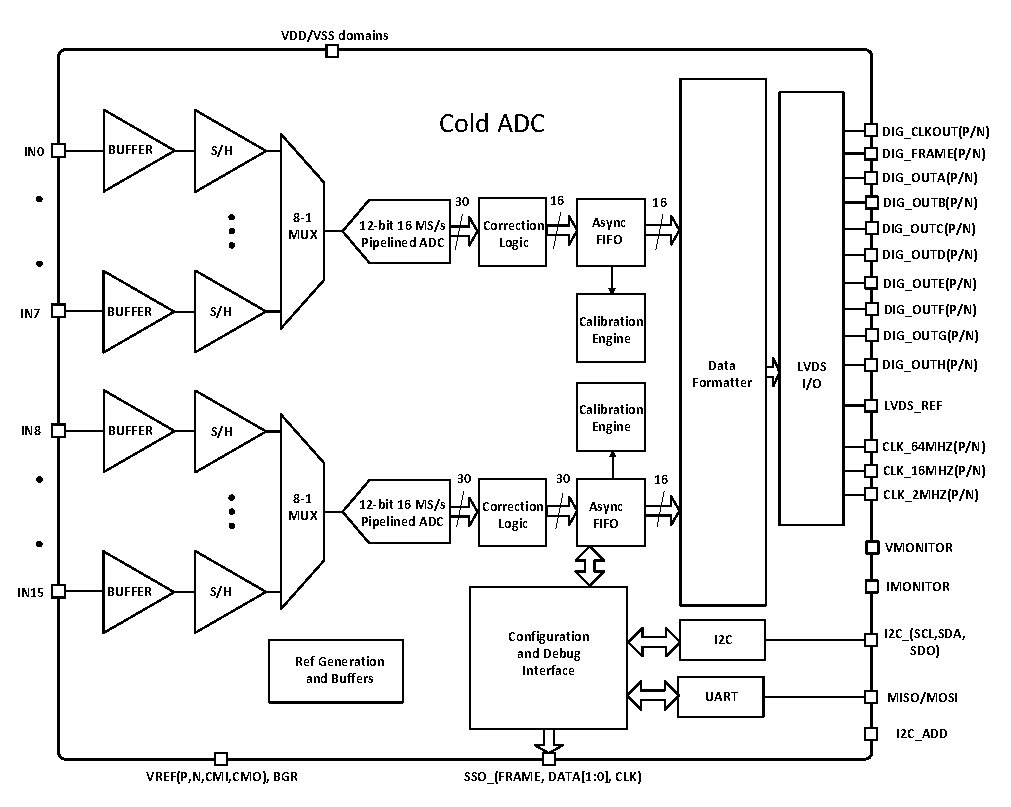
\includegraphics[width=0.75\textwidth]{tpcelec-ADCChipBlockDiagram.pdf}
\end{dunefigure}

Each Cold \dword{adc} receives \num{16} single-ended voltage outputs from a single \dword{larasic} chip. The voltage is buffered and then sampled at a rate of \SI{2}{MHz}. The analog samples are multiplexed by eight and digitized by calibrated \num{12}\,bit pipelined \dwords{adc} operating at \SI{16}{MHz}. The \dword{adc} uses the well-known pipelined architecture with redundancy to reduce the impact of component non-idealities on the linearity of the \dword{adc}~\cite{121557}. The linearity of the raw output samples from the \dwords{adc} is improved using an on-chip calibration. The corrected \dword{adc} output is then multiplexed onto eight \dword{lv}DS channels and sent to \dword{coldata} for further aggregation and transmission via a copper link to the warm electronics sitting outside the cryostat.

The \dword{adc} \dword{asic} is designed for low-noise operation. The noise specification is \SI{175}{\micro\volt} \rms. This noise specification was chosen to ensure that \dword{larasic} will dominate the overall noise performance of the channel.

The \dword{adc} is digitally calibrated using the proven Soenen-Karanicolas algorithm~\cite{280084,372864}. The algorithm exploits the observation that in a pipelined \dword{adc} with redundancy, the \dword{adc} nonlinearity is caused almost entirely by errors in the closed-loop interstage gain~\cite{121557}. Traditionally, the \dword{adc} output bits are assumed to be in radix two and are simply combined to generate the \dword{adc} output. However, due to unavoidable non-idealities such as finite op-amp gain and capacitor mismatch, the true radix of each stage is slightly different from two. The extent to which the true radix is different from two leads to DNL and INL in the \dword{adc} transfer characteristic. The Soenen-Karanicolas algorithm provides a way to measure the radix of a given stage by forcing events at the decision boundaries and using the following stages of the \dword{adc} to record the stage's response. The radix is then decomposed into a set of weights and during normal operation the \dword{adc} output is converted from the true radix to radix two using pipelined digital adders. This way, static linearity can be greatly improved without any post-processing required. To provide additional ease-of-use, all calibration hardware (including test signal generation) is included on the \dword{adc} \dword{asic}. To control power dissipation, the stages of the \dword{adc} are scaled in area to take advantage of the fact that the accuracy requirements of the stages decline down the pipeline~\cite{494191}.

To reduce the number of pads and to improve performance all required reference voltages and currents are generated internally by a resistor-programmed reference generator on the \dword{asic}.

The cold \dword{adc} is highly configurable (see Table~\ref{tab:adcconfig}) and includes two redundant slow control interfaces for configuration (either UART or I2C). The configurability of the chip is included primarily to reduce risk by providing a high degree of flexibility and observability. First, many of the components on the \dword{asic} can be bypassed and their functions assumed at the board level if desired. For example, the \dword{adc} reference voltages can be supplied externally and the input buffers can be bypassed. Second, the \dword{adc} digital calibration algorithm can be implemented externally with the calculated stage weights loaded back into the chip using the configuration interface. Third, various internal voltages and currents can be monitored and test data can be introduced at various parts of the digital processing to observe the function of the \dword{asic}. Lastly, the bias point of the analog circuits in the \dword{asic} can be adjusted to compensate for expected component variations between room temperature and \lar temperature.

\begin{dunetable}
[Baseline cold \dword{adc} \dword{asic} configurability.]
{p{3cm} p{9cm} p{4cm}}
{tab:adcconfig}
{Baseline Cold \dword{adc} \dword{asic} configurability.}
\textbf{BLOCK} &\textbf{Configurability} & \textbf{Comment}\\ \toprowrule
Input Buffer & Single-ended/differential, bypass, bias current adjust & Reduces design risk \\ \colhline
Sample-and-hold Amplifiers & Multiplexer freeze, bias current adjust & Simplifies evaluation of prototype \\ \colhline
\dword{adc} & Bias currents, clock edge fine adjustment, sync and test modes & Simplifies evaluation of prototype and reduces risk \\ \colhline
References & All reference voltages can be adjusted in \SI{8}{mV} increments; all references can be powered down and external voltages used & Reduces design risk \\ \colhline
Calibration & Number of stages and amount of digital filtering; all calibration commands can be implemented through configuration interface for offline calibration; known data can be injected at various points for testing & Simplifies evaluation of prototype and reduces risk \\ \colhline
Output Monitor & Various internal bias voltages and currents can be sent off-chip for evaluation & Simplifies evaluation of prototype \\
\end{dunetable}

%References:
%[1] S.H. Lewis, H.S. Fetterman, G.F. Gross, R. Ramachandran, and T.R. Viswanathan, “A 10-b 20-Msample/s analog-to-digital converter,” IEEE J. Solid-State Circuits, vol. 27, no. 3, pp. 351–358, March 1992.
%[2] A.N Karanicolas, H.S. Lee, and K.L. Bacrania, “A 15-b 1-Msample/s digitally self-calibrated \dword{adc},” IEEE J. Solid-State Circuits, vol. 28, no. 12, pp. 1207–1215, December 1993.
%[3] E.G. Soenen and R.L. Geiger, “An architecture and an algorithm for fully digital correction of monolithic pipelined \dwords{adc},” IEEE Trans. Circuits Syst. II, vol. 42, no. 3, pp. 143–153, March 1995.
%[4] D.W Cline and P.R. Gray, “A power optimized 13-b 5 Msamples/s pipelined analog-to-digital Converter in 1.2 µm \dword{cmos},” IEEE J. Solid-State Circuits, vol. 31, no. 3, pp. 294–303, March 1996.
